\documentclass[tikz,border=5mm]{standalone}
\usepackage{tikz}
\usepackage{amsmath}

\usetikzlibrary{arrows.meta, positioning, calc}

\colorlet{colour_c}{gray!70!black}
\definecolor{colour_n}{HTML}{3680c4}
\colorlet{colour_o}{red!90!black}

\begin{document}

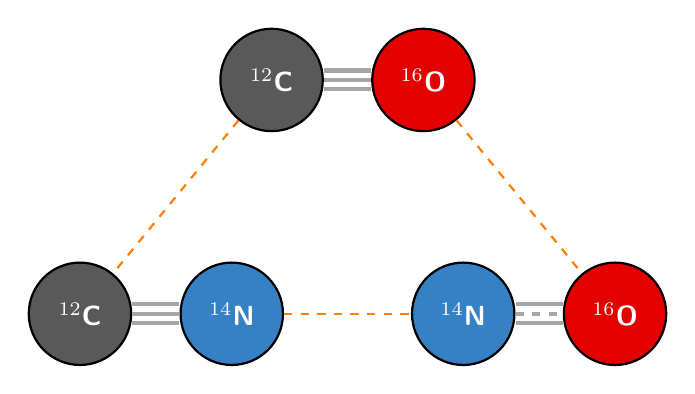
\begin{tikzpicture}
   [
      atom/.style={circle, draw, thick, minimum size=1.3cm, font=\sffamily\bfseries\color{white}},
      bond/.style={line width=1.5pt, gray!70},
      label node/.style={text=black, font=\sffamily\small},
      node distance=1cm and 2.5cm % Vertical and Horizontal spacing
   ]

   % =======================================================
   % Top Molecule: CO (12C, 16O)
   % =======================================================

   % Position C_CO at (0,0)
   \node[atom, fill=colour_c] (C_CO) at (0,0) {$^{12}\text{C}$};
   \node[atom, fill=colour_o, right=0.6cm of C_CO] (O_CO) {$^{16}\text{O}$};

   % Triple bond
   \draw[bond] ($(C_CO.east) + (0,0.12)$) -- ($(O_CO.west) + (0,0.12)$);
   \draw[bond] (C_CO) -- (O_CO);
   \draw[bond] ($(C_CO.east) - (0,0.12)$) -- ($(O_CO.west) - (0,0.12)$);

   % Midpoint coordinate for centring labels
   \path let \p1 = (C_CO), \p2 = (O_CO) in
      coordinate (mid_top) at ($(\p1)!.5!(\p2)$);

   % =======================================================
   % Bottom Left Molecule: CN (12C, 14N)
   % =======================================================

   % Position relative to Top Molecule (Down and Left)
   \node[atom, fill=colour_n, below left=2.5cm and 1cm of mid_top] (N_CN) {$^{14}\text{N}$};
   \node[atom, fill=colour_c, left=0.6cm of N_CN] (C_CN) {$^{12}\text{C}$};
   
   % Triple bond
   \draw[bond] ($(C_CN.east) + (0,0.12)$) -- ($(N_CN.west) + (0,0.12)$);
   \draw[bond] (C_CN) -- (N_CN);
   \draw[bond] ($(C_CN.east) - (0,0.12)$) -- ($(N_CN.west) - (0,0.12)$);

   % =======================================================
   % Bottom Right Molecule: NO (14N, 16O)
   % =======================================================
   
   % Position relative to Top Molecule (Down and Right)
   \node[atom, fill=colour_n, below right=2.5cm and 1cm of mid_top] (N_NO) {$^{14}\text{N}$};
   \node[atom, fill=colour_o, right=0.6cm of N_NO] (O_NO) {$^{16}\text{O}$};

   % 2.5 bond
   \draw[bond] ($(N_NO.east) + (0,0.12)$) -- ($(O_NO.west) + (0,0.12)$);
   \draw[bond, dashed] (N_NO) -- (O_NO);
   \draw[bond] ($(N_NO.east) - (0,0.12)$) -- ($(O_NO.west) - (0,0.12)$);

   % =======================================================
   % Arrows (Straight lines)
   % =======================================================
    
   % O to O (Top Right to Bottom Right)
   \draw[-, thick, orange, dashed] (O_CO) -- (O_NO);

   % C to C (Top Left to Bottom Left)
   \draw[-, thick, orange, dashed] (C_CO) -- (C_CN);

   % N to N (Bottom Middle connection)
   \draw[-, thick, orange, dashed] (N_CN) -- (N_NO);

\end{tikzpicture}

\end{document}